
\subsection{A Review of VIO/VSLAM Models}
This section reviews classical vision technique-based VIO/VSLAM models, focusing on established pipelines that rely on feature extraction, geometric constraints, and optimization or filtering to estimate motion and map structure.

\subsubsection{openVINS}
OpenVINS (Open Visual-Inertial Navigation System) is an open-source, filter-based visual–inertial odometry (VIO) framework developed for real-time state estimation in robotics, UAVs, and AR/VR applications. The system is built upon the Multi-State Constraint Kalman Filter (MSCKF) framework, where the state vector consists of IMU pose, velocity, inertial biases, and a sliding window of historical camera poses. Instead of explicitly estimating 3D landmarks, OpenVINS leverages multi-view feature constraints to update the state efficiently[1]. High-rate IMU measurements are used for state propagation, while visual measurements are incorporated through feature tracking (typically KLT optical flow) and RANSAC-based outlier rejection. The framework is implemented in modern C++ with ROS integration, OpenCV for image processing, and Eigen for linear algebra operations. Experimental evaluations on datasets such as EuRoC MAV demonstrate competitive accuracy with low translational drift (approximately 1–3\%)\cite{openvins} while maintaining real-time performance on CPU-only systems.

\noindent\textbf{Advantages:} Efficient MSCKF filtering enables real-time, CPU-only deployment; the pipeline is modular and supports online camera--IMU extrinsic and time-offset calibration.

\noindent\textbf{Disadvantages:} No built-in loop closure or persistent mapping, so drift accumulates over long trajectories; performance depends on reliable feature tracking and degrades in low-texture or visually degraded scenes.

\subsubsection{ORB-SLAM3}
ORB-SLAM3 is a state-of-the-art, open-source visual (and visual–inertial) simultaneous localization and mapping (SLAM) system designed for accurate and globally consistent pose estimation in robotics, AR/VR, and autonomous navigation applications. It extends the ORB-SLAM family by supporting monocular, stereo, RGB-D, and visual–inertial configurations within a unified framework\cite{orbslam3}. The system follows a keyframe-based, optimization-driven architecture built around ORB (Oriented FAST and Rotated BRIEF) features for robust and efficient feature extraction and matching.
The core architecture consists of three parallel threads: Tracking, Local Mapping, and Loop Closing. The Tracking thread extracts ORB features, estimates camera pose via motion models and Perspective-n-Point (PnP) optimization, and decides keyframe insertion. The Local Mapping thread performs local bundle adjustment (BA) to optimize poses and 3D landmarks within a sliding window of keyframes. The Loop Closing thread detects place revisits using bag-of-words (BoW) place recognition and performs pose graph optimization and full bundle adjustment to ensure global consistency.
In visual–inertial mode, ORB-SLAM3 tightly integrates IMU measurements using preintegration theory and performs joint optimization over visual and inertial states. The system is implemented in C++ and relies on OpenCV for image processing, Eigen for linear algebra, DBoW2 for place recognition, and g2o for nonlinear graph optimization. Evaluations on benchmark datasets such as EuRoC MAV and TUM-VI demonstrate high accuracy with strong global consistency, often outperforming previous ORB-SLAM versions and many contemporary SLAM systems.

\begin{figure}[H]
    \centering
    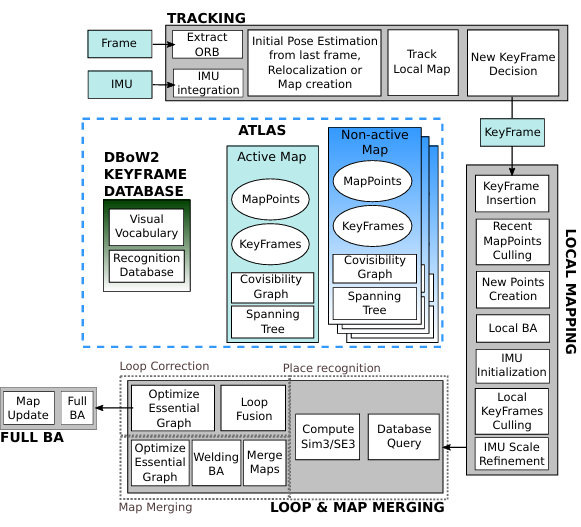
\includegraphics[width=0.8\textwidth]{images/orbslam3.png}
    \caption{ORB-SLAM3 Architecture \cite{orbslam3}.}
    \label{fig:orblsma3_architecture}
\end{figure}

\begin{itemize}
    \item \textbf{Advantages:} ORB-SLAM3 achieves high global accuracy by combining robust place recognition with loop closing and full bundle adjustment, which significantly reduces drift over long trajectories. It supports monocular, stereo, RGB-D, and tightly coupled visual--inertial configurations and maintains a persistent, reusable map for long-term and multi-session localization.
    \item \textbf{Disadvantages:} Its optimization-heavy pipeline (bundle adjustment and pose-graph optimization) increases CPU and memory requirements relative to filter-based systems, and the multi-threaded architecture adds implementation and tuning complexity. Additionally, monocular and visual--inertial initialization can be sensitive to motion conditions, making early-stage tracking less reliable in some scenarios.
\end{itemize}

\subsubsection{PyCuVSLAM}
PyCuVSLAM is a Python interface for the CUDA‑accelerated visual SLAM (cuVSLAM) library developed by NVIDIA Research, providing high‑performance visual odometry and SLAM capabilities with GPU acceleration. PyCuVSLAM wraps the underlying cuVSLAM C++/CUDA implementation in a Python API, allowing real‑time processing of visual data from monocular, stereo, RGB‑D, multicamera, and visual–inertial (IMU) configurations with low latency and high throughput. The system leverages NVIDIA GPUs (via CUDA) to accelerate feature tracking, pose estimation, mapping, and loop closure tasks, making it suitable for demanding robotics, UAV, and perception applications where CPU‑only SLAM may be too slow\cite{cuvslam}. PyCuVSLAM supports ROS2 integration and example workflows for standard datasets such as EuRoC and KITTI, and produces camera pose estimates, sparse maps, and other SLAM outputs in real time. Its design emphasizes computational efficiency through parallel CUDA kernels while exposing a user‑friendly Python interface suitable for rapid prototyping and research. 

\begin{figure}[H]
    \centering
    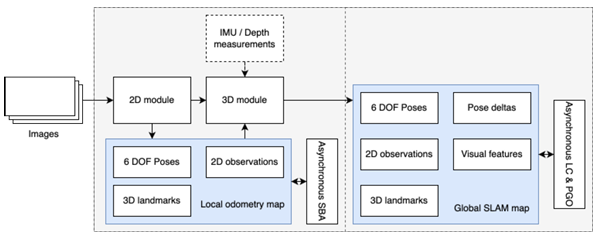
\includegraphics[width=0.8\textwidth]{images/cuvslam.png}
    \caption{cuVSLAM Architecture \cite{cuvslam}.}
    \label{fig:cuvslam_architecture}
\end{figure}

\begin{itemize}
    \item \textbf{Advantages:} CUDA acceleration enables high-throughput, low-latency SLAM that can outperform many CPU-only pipelines, while the Python API and ROS2 support simplify prototyping and integration. It supports multiple sensing setups, including RGB-D, IMU (visual--inertial), and multicamera configurations.
    \item \textbf{Disadvantages:} It depends on NVIDIA CUDA-capable GPUs and is distributed under a non-commercial NVIDIA license, limiting portability and commercial deployment. Setup can be complex due to CUDA/ROS2 dependencies, and the system has comparatively limited peer-reviewed validation (primarily an arXiv reference).
\end{itemize}

\subsubsection{Qualcomm qVIO}
 Qualcomm qVIO (Qualcomm Visual–Inertial Odometry) is a proprietary visual–inertial tracking solution developed by Qualcomm for real-time pose estimation on mobile and embedded platforms powered by Qualcomm Snapdragon processors. It is designed primarily for augmented reality (AR), virtual reality (VR), robotics, and mobile perception applications where low latency and power efficiency are critical.
qVIO performs tightly coupled fusion of camera and inertial measurement unit (IMU) data to estimate 6-DoF pose. The system leverages Qualcomm’s heterogeneous computing architecture, utilizing the CPU, GPU, and Digital Signal Processor (DSP) (e.g., Hexagon DSP) to accelerate visual feature processing and inertial fusion. The architecture typically consists of image feature extraction and tracking, IMU propagation, sensor fusion via nonlinear filtering or optimization-based methods, and drift correction mechanisms. The design emphasizes low-power real-time performance suitable for mobile SoCs rather than desktop-class systems.
qVIO has been widely used in Snapdragon-based development platforms such as Qualcomm’s Robotics RB-series and earlier AR/VR reference devices. Performance characteristics generally include low-latency tracking, robustness under moderate motion, and hardware-accelerated execution optimized for Snapdragon chipsets.\cite{qvio}

\begin{figure}[H]
    \centering
    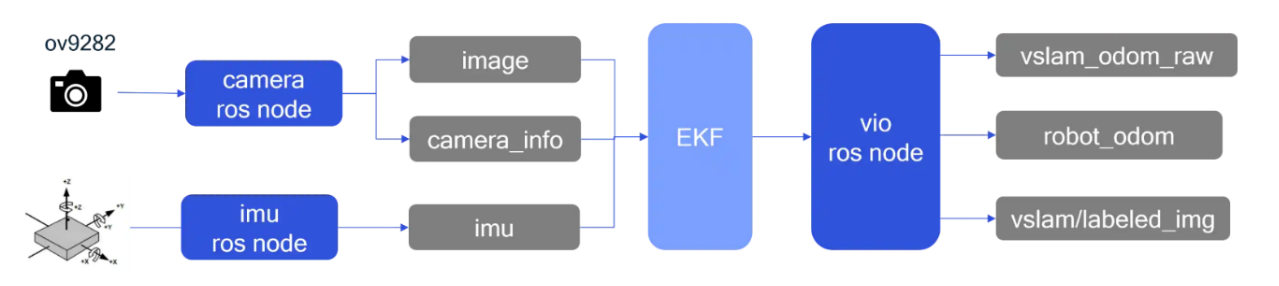
\includegraphics[width=0.8\textwidth]{images/qualcom_qvio.png}
    \caption{qVIO pipeline \cite{qvio}.}
    \label{fig:qvio_pipeline}
\end{figure}

\begin{itemize}
    \item \textbf{Advantages:} It directly mitigates the primary failure mode of traditional SLAM by robustly handling dynamic environments. This results in a significant boost in localization accuracy and system robustness in real-world scenarios, while maintaining the real-time performance of the underlying ORB-SLAM3 framework.
    \item \textbf{Disadvantages:} Its effectiveness is fundamentally limited by the capabilities of the object detector. It cannot handle moving objects that do not belong to one of its known classes, and its performance may degrade if the detector is not robust to different viewpoints or lighting conditions.
\end{itemize}

\subsubsection{Summary}

\begin{table}[H]
\centering
\scriptsize % reduces font size
\caption{Comparison of VIO Algorithms}
\resizebox{\textwidth}{!}{%
\begin{tabular}{|p{1.6cm}|p{1.9cm}|p{1.4cm}|p{1.9cm}|p{4.1cm}|p{4.1cm}|}
\hline \textbf{Algorithm} & \textbf{Core Method} & \textbf{Coupling} & \textbf{Camera Support} & \textbf{Key Innovations \& Strengths} & \textbf{Key Limitations \& Challenges} \\

\hline openVINS & Filter-based (EKF/MSCKF) & Tightly & Monocular, Stereo &
\begin{itemize}[leftmargin=*, topsep=0pt, itemsep=0pt, parsep=0pt, partopsep=0pt]
  \item Open-source, modular EKF-based VIO with MSCKF-style feature handling.
  \item Real-time on embedded platforms; flexible sensor/feature front-end.
  \item Well-suited for research comparisons and UAV implementations.
\end{itemize} &
\begin{itemize}[leftmargin=*, topsep=0pt, itemsep=0pt, parsep=0pt, partopsep=0pt]
  \item Generally lower accuracy than optimization-based smoothing methods.
  \item Requires careful tuning/calibration for best consistency.
  \item No native global map reuse/loop closure (drift over long trajectories).
\end{itemize} \\

\hline ORB-SLAM3 & Optimization-based (MAP/BA, SLAM) & Tightly & Monocular, Stereo, RGB-D &
\begin{itemize}[leftmargin=*, topsep=0pt, itemsep=0pt, parsep=0pt, partopsep=0pt]
  \item Visual--inertial SLAM with relocalization, loop closure, and multi-map (Atlas).
  \item Strong accuracy and long-term robustness for re-visitation / tracking loss.
\end{itemize} &
\begin{itemize}[leftmargin=*, topsep=0pt, itemsep=0pt, parsep=0pt, partopsep=0pt]
  \item Heavyweight SLAM system (complexity and compute) vs.\ pure odometry.
  \item Integration/tuning overhead can be high for constrained UAV stacks.
\end{itemize} \\

\hline cuVSLAM (pycuVSLAM) & GPU-accelerated VSLAM/VIO & Tightly & Mono, Stereo, RGB-D, +IMU &
\begin{itemize}[leftmargin=*, topsep=0pt, itemsep=0pt, parsep=0pt, partopsep=0pt]
  \item CUDA-accelerated pipeline enables low-latency, high-throughput tracking.
  \item Python API and ROS2 integration simplify prototyping.
  \item Supports IMU and multi-camera configurations.
\end{itemize} &
\begin{itemize}[leftmargin=*, topsep=0pt, itemsep=0pt, parsep=0pt, partopsep=0pt]
  \item Requires NVIDIA CUDA-capable GPU (portability constraints).
  \item Licensing can restrict commercial deployment.
  \item Limited peer-reviewed benchmarking relative to academic baselines.
\end{itemize} \\

\hline Qualcomm qVIO & Proprietary VIO (mobile SoC) & Tightly & Monocular (typical) &
\begin{itemize}[leftmargin=*, topsep=0pt, itemsep=0pt, parsep=0pt, partopsep=0pt]
  \item Optimized for Snapdragon platforms (CPU/GPU/DSP acceleration) with low power.
  \item Low-latency 6-DoF tracking for AR/VR and embedded robotics use.
\end{itemize} &
\begin{itemize}[leftmargin=*, topsep=0pt, itemsep=0pt, parsep=0pt, partopsep=0pt]
  \item Closed-source/proprietary; limited transparency and academic validation.
  \item Platform-locked to Qualcomm ecosystem and supported devices.
\end{itemize} \\

\hline \end{tabular}}
\label{tab:VINS_comparison}
\end{table}

\subsubsection{Justification for Choosing ORB-SLAM3}
After comparing VIO/VSLAM models, ORB-SLAM3 was selected as the primary baseline for this project.
\begin{itemize}
    \item Provides strong global consistency through loop closure and full bundle adjustment.
    \item Supports monocular, stereo, RGB-D, and visual--inertial configurations within one framework.
    \item Demonstrates high accuracy on standard benchmarks and practical UAV scenarios.
    \item Offers a mature, widely adopted open-source codebase with extensive documentation.
\end{itemize}